\documentclass{article}
\usepackage{amsthm,amssymb,amsmath,mathtools,graphicx,url}
% \usepackage[margin=1in]{geometry}
% \usepackage{fancyhdr}

\title{Keeping DRY: A Comprehensive Measure of Modularity Within a Computer Program}
\author{J. Hassler Thurston}
\date{}

\begin{document}
\maketitle

\begin{abstract}

DRY, which stands for ``Don't Repeat Yourself'', is a principle in software engineering that discourages programmers from
writing duplicate code while programming. Since following the DRY principle has many benefits, it is important that it 
be measured. We present a few heuristics for measuring DRY, mostly followed from results of detecting
similarity between two programs. We show how these heuristics lay the foundation for future work, and how they
 may turn out useful for encouraging amateur programmers to improve their coding style.

\end{abstract}

\section{Introduction} DRY, or ``Don't Repeat Yourself'', is a programming ideal and standard that urges programmers to avoid 
duplicating code or structures of code in order to make programming more efficient and readable. It was first formulated by Andrew Hunt
 and David Thomas in 1999 in their book ``The Pragmatic Programmer'', in which they state that ``every piece of knowledge must have a 
 single, unambiguous, authoritative representation within a system''~\cite{PragmaticProgrammer}. Following DRY means writing more modular
code, which by definition means separating each part of a program into different pieces, each piece solving a specific sub-problem.
A program that does not follow the DRY principle is termed WET, which some have satirically expanded as ``write everything twice''
 and ``we enjoy typing''~\cite{WETness}.

As stated by Frederick Brooks in an article
from April 1987\cite{NoSilverBullet}, software engineering will always face four essential difficulties: complexity, conformity, 
changeability, and invisibility. Following DRY can help alleviate the troubles of complexity and changeability since breaking up code
into small pieces makes it easier to understand, and changing code that is already modular is almost by definition easy.

We thus set out to create a measure of ``DRYness'', so that we can evaluate how modular people's programs are.
By creating such a measure, we can not only analyze code in a new, objective way, but we can also try to encourage amateur programmers
to reflect on their code design and improve their coding style if necessary.

However, coming up with an objective measure is subject to many difficulties. First, we have searched the literature and have only found a few similar measures described, so we are one of the first to try to objectively define a DRYness measure.
Second, once we have a measure of DRYness,
it is hard to argue objectivity of the measure, since in some sense the way we measure modularity of code is subject to personal
interpretation. Because of these difficulties, we have chosen to take a slightly different approach. We have created several 
heuristics for measuring the modularity of code, and compare the heuristics by testing and comparing them on a number of different
hand-written programs which we feel captivate many cases of modular or non-modular design.

\section{Related Work} As stated above, we think we are one of the first ones to come up with a measure of DRYness. There have been
some attempts in the past to evaluate program modularity, which for purposes of this paper will be considered the same as program DRYness.
Baker et. al.\cite{Modularity1979} describe an approach to measure effort expended while writing a program in order
to determine when program modularity is beneficial. To Baker et. al., effort expended is defined as the ratio of program volume to 
the ``level of implementation'', which are both based on counting the number of total and distinct operands and operators in a program.
They then use their measure of effort, which they claim measures program modularity accurately, to evaluate over 500 programs to
determine when it is useful to modularize code. Ratiu et. al.\cite{LogicalModularity} develop a heuristic that determines the 
difference between how code is modularized and how it \textit{should} be modularized based on the underlying logic. However, their heuristic
evaluates program structure as a whole, meaning that they analyze packages, classes, and functions/methods (and their names) but not the 
content of these functions or methods.

Besides the two papers described above, we have found that much related work has been done on a similar topic, namely
 program similarity. That is, given two programs, we would like to know how similar they are in style to each other.
This is useful for detecting plagiarism among amateur student programmers, and detecting whether other concepts or programs
have been implemented before. Joy, Joy, and Luck \cite{PlagiarismProgrammingAssignments} note that since much of student plagiarism involves changing a program structurally (e.g. replacing a for loop with a while loop) and lexically (e.g. rewording comments), they can
detect similarity with an incremental comparison method, whereby they study different possible modifications of two programs.
Whale \cite{ProgramSimilarityPopulations} takes a slightly different approach, whereby he counts the number of occurrences of certain attributes of programs (such as the number of unique operators and operands), and combines this metric with a similarity measure over optimized versions of code at runtime. Similar to \cite{Modularity1979}, these approaches involve counting the occurrences of certain attributes within programs, such as logical operators, operands, and keywords.

Much of the other related work\cite{McGahn1995,GraphSimilarityStudentPrograms} we have found centers on two different ideas for detecting similarity or modularity
(one of which was just described): counting occurrences
of certain attributes and detecting similarity of parse trees. Counting occurrences of certain attributes is relatively easy, as we can
determine these counts by a single pass through a program. Moreover, many people have found this approach to detect similarity 
somewhat accurately \cite{Modularity1979}\cite{PlagiarismProgrammingAssignments}. However, there are many instances when counts of
logical operators and operands could be the same, but programs could be very different. Thus the need for detecting structural similarity.

Detecting structural similarity is relatively hard, since we first must perform a lexical analysis and a parse of a program, which takes
multiple passes over a program. Once we have parse trees for programs, it is also then hard to determine which subtrees to compare for
similarity, and furthermore how to compare them. However, such an analysis can have the potential to be very useful and beneficial
for determining similarity\cite{ProgramSimilarityPopulations}\cite{PlagiarismProgrammingAssignments}.

\section{Design and Implementation}

\subsection{DRYness score and setup}

We will define the DRYness score of a program to be in the range $[0,1]$. A DRYness score close to 0 means the program is ``very dry'',
and a score near 1 means the program is ``very wet'', i.e. repetitive. A DRYness score of -1 means the Java program does not compile.

Our DRYness score is computed using Java, meaning that our heuristics only work on Java files. However, similar heuristics could 
be used to detect DRYness for most other programming languages. We chose to implement our heuristics for Java files since Java 
is a popular programming language among amateur programmers, and we found a convenient external library to lexically analyze and parse
Java files efficiently \cite{Javaparser}.

\subsection{Test dataset}

We compute the DRYness heuristics (described below) on seven different test Java files, which we feel captures the basic properties
of DRYness somewhat well. Of these seven test files, one consists of an empty class (for a baseline measurement), and the other six are paired,
three of which are simple, modular programs; and three of which are WET versions of the modular programs. We thus expect the wet versions of the pair to have a DRYness score close to 1, and the dry versions of the pair
to output a score close to 0. We also test our heuristics on our own Java programs, to give us some insight on how well our DRYness
programs are in themselves modular, and to see how our heuristics perform on larger Java programs. By testing whether our heuristics return relevant values on these files, we can somewhat objectively evaluate the success of our heuristics.

\subsection{Heuristics}

We have so far implemented five heuristics (four non-trivial ones) and tested them on our test dataset. These heuristics have varying levels of success
and employ various techniques to evaluate DRYness structurally. Our trivial heuristic always returns a DRYness score of 0 (for a
baseline).

\paragraph{Modified Baker Heuristic}
We decided to implement a modification of an early heuristic that was used to measure program modularity.
As outlined by Baker et. al. \cite{Baker1979}, the Modified Baker Heuristic involves considering the ratio of distinct operators and operands to the total number of operators and operands. However, we were not able to implement this in its entirety, since the difficulty
of getting accurate counts of each instance of an operator and an operand is somewhat beyond the scope of the Javaparser library.
Therefore, we modified the heuristic to compute the ratio of distinct operator and operand \textit{types} to the total number of
operators and operands. For example, our program will not distinguish between instances of \texttt{+}, \texttt{-}, \texttt{*}, and \texttt{/}, since these are all arithmetic operators. Since there are a very limited number of operator types, we suspect that this
heuristic may skew the DRYness score.

Since this ratio will be relatively small for modular Java files, we decided to take the difference between 1 and this ratio as the modified Baker heuristic's DRYness score. For more explanation on why this is the case, please see the Results section.

We must note that the heuristic proposed in \cite{Baker1979} is therefore significantly different than the heuristic we implemented.
This paper explores a concept of program volume, which is computed somewhat differently than this ratio.

\paragraph{Iteration 1 Heuristic}

The Iteration 1 Heuristic defins DRYness recursively, 
starting from the root node of a program's parse tree. For the heuristic to be well-defined, we must define the DRYness score of
each type of parse tree node, and output a number between 0 and 1. For example, our definition of the DRYness score of an if statement
will be defined differently than the DRYness score of a variable assignment statement. Thus, for each type of parse tree node,
the Iteration 1 Heuristic mostly computes the average of the DRYness scores for each sub-tree of a given node. For trivial parse
tree nodes, the Iteration 1 Heuristic returns either 0 or 1. Furthermore, for a given Block Statement (comprising a sequence of statements), 
the Iteration 1 Heuristic compares each statement pairwise for equality. If there are pairs of statements that are equal, the 
heuristic increases the DRYness score by a small amount, equal to $1/\#totalPairs$. Note that this will keep the DRYness score
less than 1, since we can only perform this increase once for each pair of statements we consider.

\paragraph{All Pairs Naive Heuristic}

The second non-trivial heuristic, the All Pairs Naive Heuristic, computes DRYness iteratively. 
For each parse tree node that the heuristic visits, it first adds the node and its contents to an \texttt{ArrayList} of other similar
parse tree nodes. This means that after visiting all nodes in a parse tree, the heuristic has a sequence of \texttt{ArrayList}s
in memory, with each \texttt{ArrayList} comprising all subtrees of a given type. The heuristic then compares the elements of each
ArrayList pairwise, checking for equality. The final DRYness score is taken to be the average of the results of the pairwise equality checks,
where each pairwise equality check is computed as follows: $$\frac{\#equalPairs}{\#totalPairs}$$, where $\#equalPairs$ is the
number of pairs of subtrees of a given type that are the same, and $\#totalPairs$ is the total number of pairwise comparisons made
for a given type of node. Note that this will also give a score of at most 1, as there will be at least as many total pairs of statements
as equal pairs of statements.

\paragraph{All Pairs Weighted Heuristic}

The third non-trivial heuristic, the All Pairs Weighted Heuristic, is a slightly modified version of the All Pairs Naive Heuristic.
Similar to the All Pairs Naive Heuristic, this heuristic compares parse tree nodes of a given type in pairs, checking for equality.
However, the All Pairs Weighted Heuristic weights each type of equality check differently, so that, for example, equal statements
within a Block Statement are penalized more heavily than equal comment strings. It thus returns a weighted average of the result
of each pairwise equality check.

\paragraph{Tree Edit Distance Heuristic}
We have not implemented a Tree Edit Distance heuristic as originally proposed, given the complexity of implementing such a heuristic. Given two subtrees, the tree edit distance between these two
trees is defined to be the number of insertions, deletions, or renaming of nodes in one tree such that the trees are
identical\cite{TreeEditDistance}. Thus, a tree edit distance of 0 implies that the two trees are equal.

We were not able implement this heuristic for two reasons. First, this heuristic is not well-defined for subtrees that are not of the same type: for example, we cannot compute the tree edit 
distance between an if statement and a comment. Second, this heuristic involves writing a rather involved algorithm if we were to compute tree edit distance efficiently, which we determined to be outside the scope of this paper. We do, however, propose to implement
such a heuristic in a successive rendition of this paper.

\section{Results}

Our results are shown in Figures \ref{fig:test} and \ref{fig:dry}. In Figure \ref{fig:test}, we graph the DRYness score for each of the five heuristics we implemented, relative to the seven example files we wrote. For Figure \ref{fig:test}, we graph
the DRYness score for each of the heuristics against our six Java files that we implemented for computing DRYness. We decided to
graph our heuristics against our implementation itself because we wanted to see how well the DRYness heuristics worked on larger
files, and because we wanted to get a somewhat objective measurement on how modular our own code was.

\paragraph{Modified Baker Heuristic}
Throughout both figures, we notice that the Modified Baker Heuristic tends to significantly give poorer ratings to Java files
than our other heuristics. This is especially true in larger Java files, most notably those of our own implementation. We can attribute this to the definition we used for the Modified Baker Heuristic: one minus the ratio of the total number of distinct operator and operand types and the total number of operators and operands.
Since there are a relatively small number of types of operators and operands, it makes sense that larger files will tend to repeat
operators and operands throughout the file. We can therefore see that our modified version of the heuristic presented in \cite{Baker1979}
may not be a good heuristic for evaluating the DRYness of files themselves. We suggest modifying this heuristic to account for the length
of the file in future work, so as to not bias the results for larger files.

\paragraph{Iteration 1 Heuristic}
We can see in Figure \ref{fig:test} that the Iteration 1 Heuristic generally gives poorer ratings to our sample files than the All Pairs Heuristics, and in Figure \ref{fig:dry} that this heuristic gives better ratings to our files than the All Pairs Heuristics. Furthermore, this heuristic
does not notice a stark difference between the two versions of DoubleFor and Factorial, and only notices a significant difference with the HelloWorld files. We can attribute this to this heuristic only checking for equality of block statements, and not other types of statements.
As somewhat rightly named, this heuristic was our first iteration at measuring DRYness, and we can conclude that the heuristic misses
some important differences between files.

\paragraph{All Pairs Naive Heuristic}
The All Pairs Naive Heuristic also shows a difference in results between larger files and smaller files. In Figure \ref{fig:test}, we
can see that the heuristic generally gives better ratings than the All Pairs Weighted Heuristic, and in Figure \ref{fig:dry}, the opposite happens. We did not expect to see this contrast between different lengths of files, and are still trying to deduce a definitive answer as to why this happens. One possible explanation is that with larger files, the proportion of pairs of statements that are exactly
equal is relatively low, whereas the opposite is the case for smaller files. The difference between this heuristic's evaluations of pairs of DRY-WET example files is rather alarming, as it does not detect a significant difference in modularity. This is partially why we
created the weighted version of this heuristic.

\paragraph{All Pairs Weighted Heuristic}
For the seven example files, we can see that the All Pairs Weighted Heuristic detects a large difference between the HelloWorld and the DoubleFor pairs of files, but not the Factorial pair. Quite shockingly, this heuristic weights the FactorialWet file as more DRY than the Factorial file! We can partially attribute this to the way these three pairs of files are structured, with the FactorialWet file having more subtle repetitive differences than the other two WET files.

Similar to the All Pairs Naive Heuristic, this heuristic generally rates Java files as DRY -- i.e. the heuristic gives low DRYness scores.
We do not think the exact weights used in the implementation of this heuristic account for this trend, but rather think that a
correction factor should be created, that accounts for the length of the Java file. This way, the All Pairs Weighted Heuristic can
more thoroughly detect the difference between large DRY Java files and large WET Java files. We have not, however, come up with 
such a correction factor that may help, as there are many possible corrections that can be performed. Implementing these correction
factors is a subject for future research.


% results for the 7 test files
% templated from Joe's sample LaTeX file given in Assignment 8
\begin{figure}
\centering
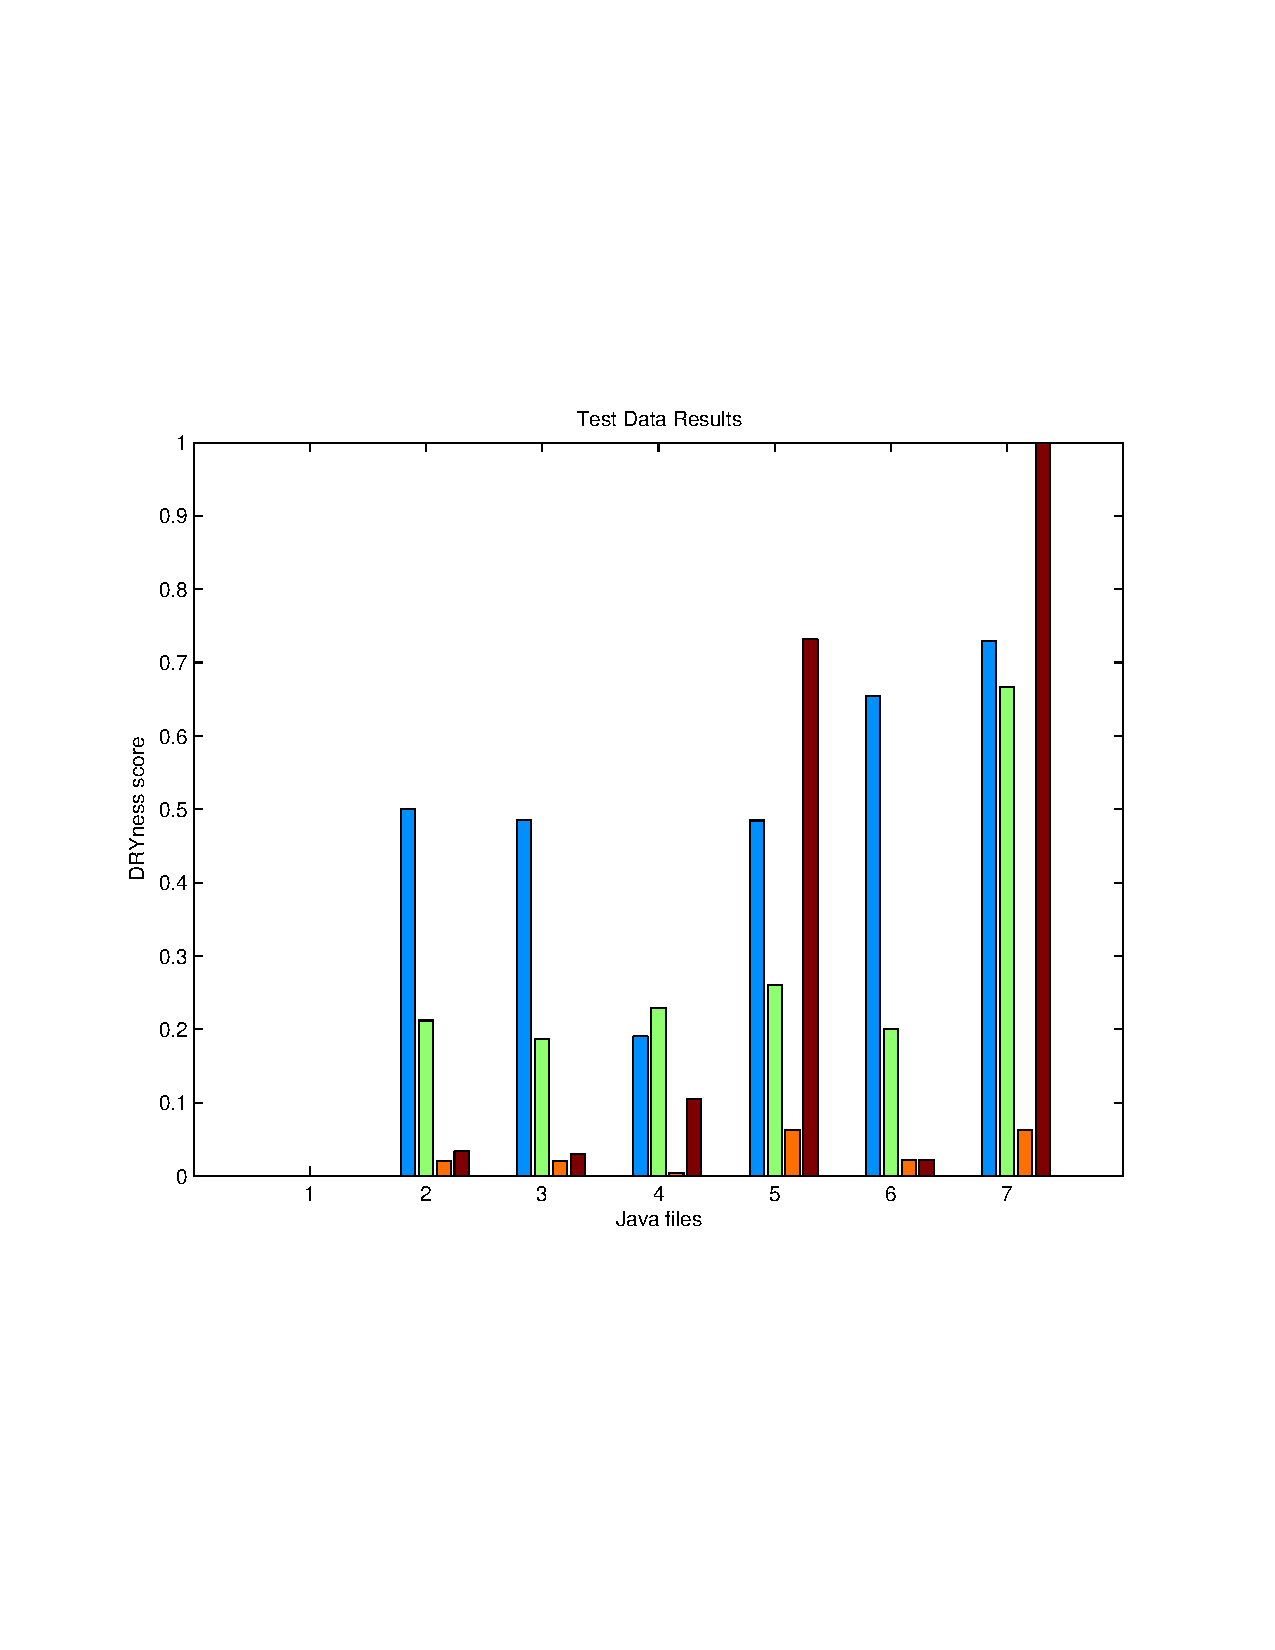
\includegraphics[clip=true, trim=0.75in 2.5in 0in 2.5in, width=3.5in]{../testPlot.pdf}
\caption{Results for the five heuristics on the seven simple test Java files. Files are ordered in increasing order of 
expected DRYness output.}
\label{fig:test}
\end{figure}
% results for our files
\begin{figure}
\centering
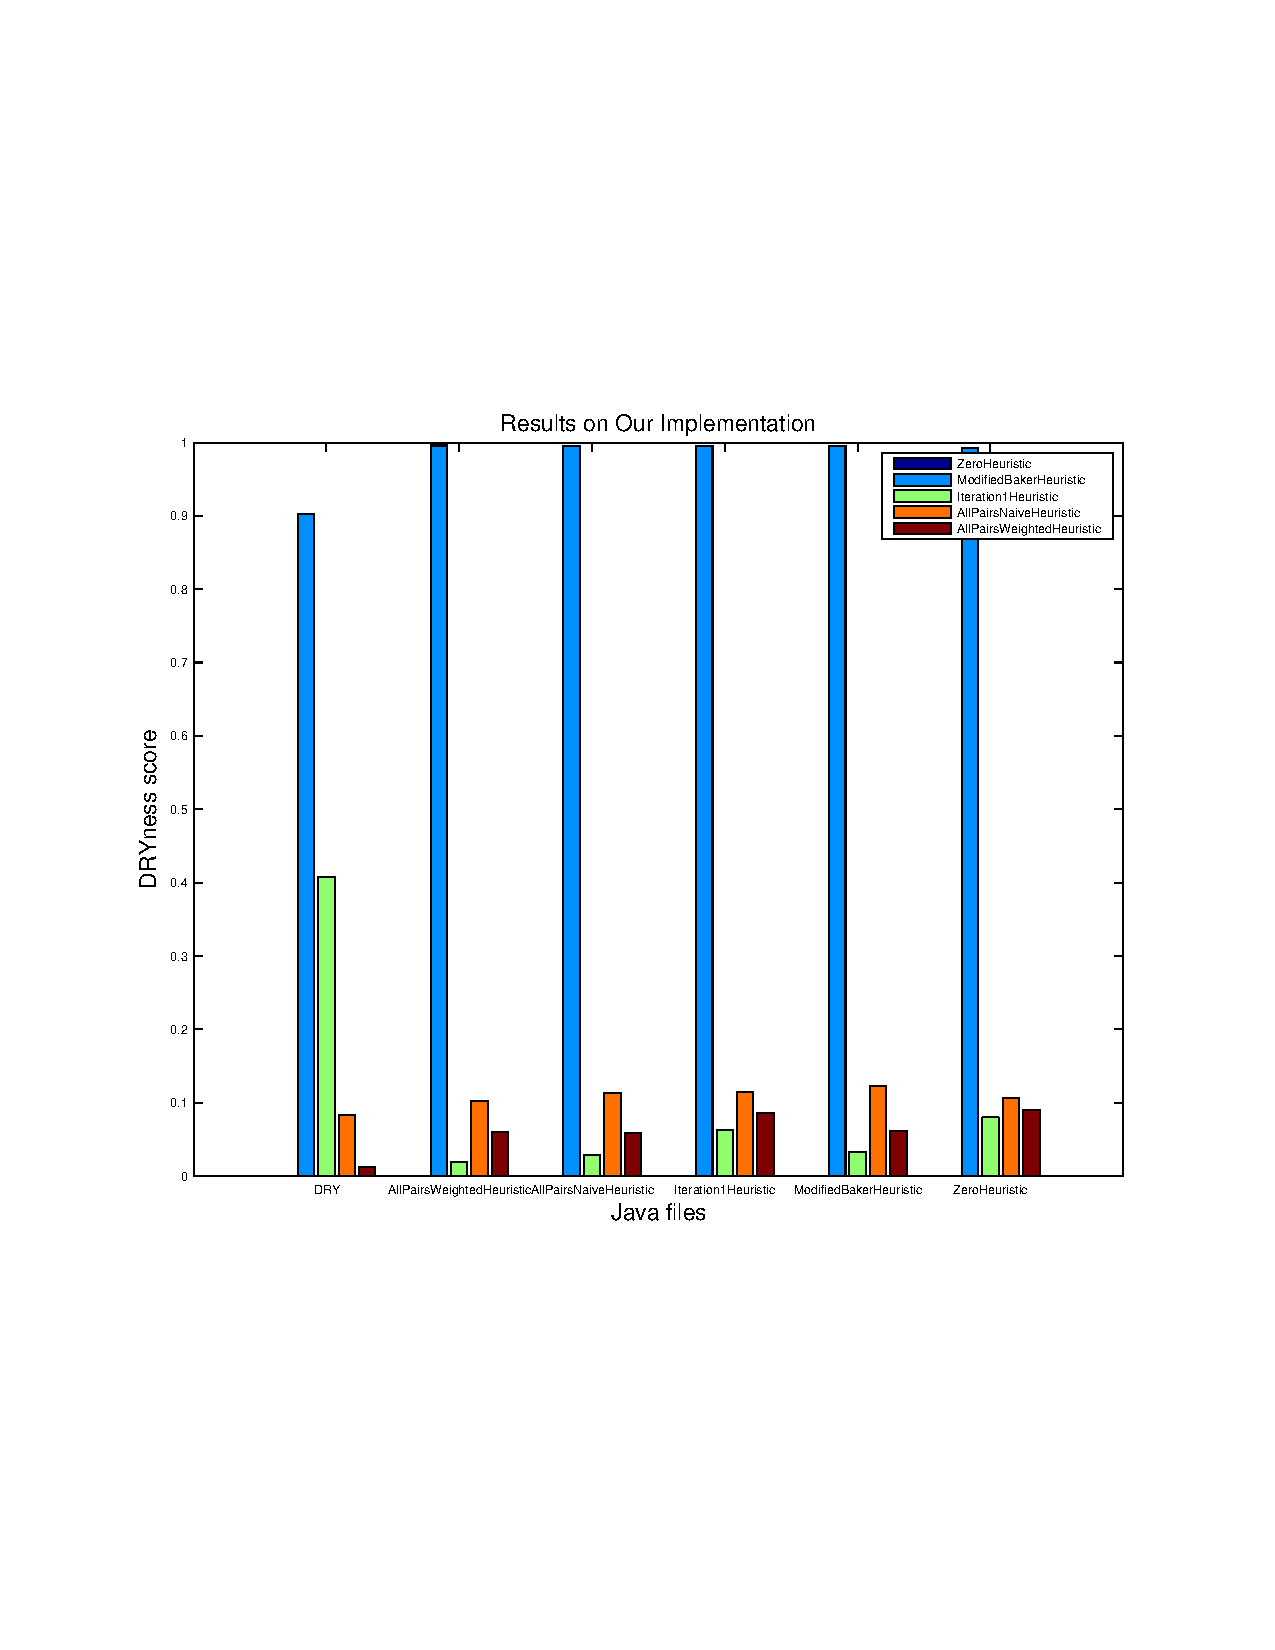
\includegraphics[clip=true, trim=0.75in 2.5in 0in 2.5in, width=3.5in]{../dryPlot.pdf}
\caption{Results for the five heuristics on our six implementation files. Files are ordered in increasing order of 
expected DRYness output.}
\label{fig:dry}
\end{figure}

\section{Conclusion and Future Work}

Evaluating the DRYness of a program or its degree of modularity is currently considered to be an unsolved problem,
even though there has been a lot of research on a similar aspect of program similarity -- that is, examining two
different programs for plagiarism detection. Similar to a couple of earlier heuristics, our heuristics involve
computing the structural similarity of a Java program by examining the similarity between subtrees of a given Java parse tree. 
We have compared these heuristics against each other, and concluded that the heuristics compute a measure of DRYness to a 
somewhat accurate extent. In particular, we have found that the All Pairs heuristics tend to outperform the Modified Baker Heuristic
and the Iteration 1 Heuristic. However, we have also seen how our heuristics can perform poorly on larger Java files, such as our
own implementation files. Many correction factors can be implemented, and more work must be done to verify which corrections
perform most optimally.

In addition to modifying these heuristics, there is still much work to be done before any DRYness heuristics can be deemed objectively
accurate. First, as noted above, we have tested our heuristics on only 13 Java files, which might have given us skewed results. A more
comprehensive evaluation of our metrics must include testing them on a plethora (possibly hundreds) of Java files, to verify whether
the general trends we observed hold for more general Java programs. Second, we would like to see whether a Tree Edit Distance heuristic
gives us more accurate results than any of our implemented heuristics. We hypothesize this will be the case, but as stated above, 
implementing a Tree Edit Distance heuristic is a relatively hard endeavor. Third, we would like to observe the performance of our
heuristic on student assignments, to see whether student grades are correlated with the modularity of their implementations. This would not only give us more Java files with which to test our heuristics, but would also start to give us an idea on whether
the DRYness metrics we computed could be implemented in practice. These facts, along with the partial success of our heuristics, is why
we consider the problem of determining how much a programmer follows the ``Don't Repeat Yourself'' principle to still be open.

\section{Acknowledgements}

The author is deeply indebted to Chen Ding and Joe Izraelevitz for their support, suggestions, and guidance over the past two months.
The author would also like to thank Victor Liu, Jacob Bisnett, Ben O'Halloran, Evan McLaughlin, Brandon Allard, and the rest of
the CSC200 student body for their recommendations, and Tyler Hannan for his help with Java generics, Unicode support issues, and
visitor patterns.



\pagebreak
\pagestyle{empty}

\bibliographystyle{plain}
\bibliography{report}

\end{document}